\section{Sistemas de Percepção}\label{sec:perception}

\subsection{LIDAR}

O TerraMax conta com 3 LIDARs do modelo ALASCA XT da Ibeo Automotive Systems com abertura de $220\degree$ e alcance de 80m, sendo dois frontais e um traseiro, dispostos conforme mostra a \reffig{fig:lidar}. Os dois sensores frontais possuem regiões de intersecção, em que as informações são fundidas.

\begin{figure}[h]
\centering
\subfloat{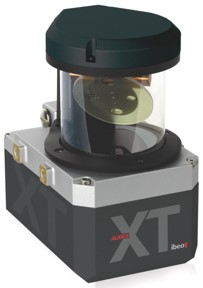
\includegraphics[height=0.35\columnwidth]{figs/lidar.jpg}}\qquad\qquad
\subfloat{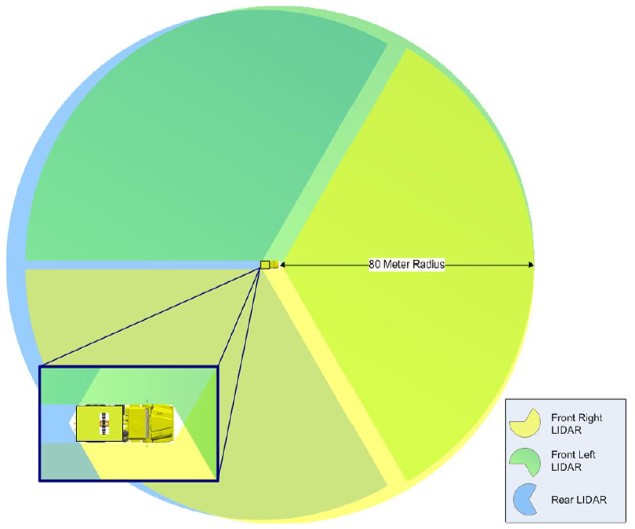
\includegraphics[height=0.35\columnwidth]{figs/laser_scan.jpg}}
\caption{Modelo de LIDAR utilizado (esq.) e região de scan (dir).}%
\label{fig:lidar}%
\end{figure}

O principal objetivo dos LIDARs é a detecção de objetos, passando essa informação já processada pelo subsistema dos LIDARs para o comportamento autônomo do sistema. Outra função é prover \emph{scans} para integração dos dados com os sistemas de imagem, aprimorando assim os resultados.

\subsection{INS}

O TerraMax utiliza um sistema de navegação inercial (INS) da Smiths Aerospace, composta por uma IMU de 6DOF integrada com informações de duas antenas GPS da Novatel e odometria das rodas em um filtro de Kalman interno \reffigp{fig:INS}. O uso de duas antenas de GPS com um baseline (distância entre as antenas) significativo de uns 2.5m aprimora as medidas de rumo da INS.

\begin{figure}[h]
\centering
\subfloat{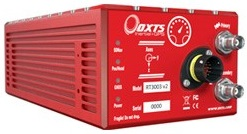
\includegraphics[height=0.25\columnwidth]{figs/INS.jpg}}\qquad
\subfloat{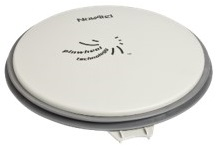
\includegraphics[height=0.25\columnwidth]{figs/antena.jpg}}
\caption{Módulo INS utilizado pelo TerraMax e uma das antenas GPS.}%
\label{fig:INS}%
\end{figure}

O objetivo da INS é naturalmente prover informações de posição absoluta no ambiente, bem como velocidades e orientações do veículo. Esses dados são utilizados no controle de trajetória juntamente com os sistemas de visão para garantir que o veículo se mantenha dentro da faixa.

Durante as etapas de teste do sistema, para efeitos comparativos da posição real do veículo com a posição estimada pelo INS, a equipe utilizou o serviço Omnistar HP, que possui precisão centimétrica.

\subsection{Sistemas de Visão}

O sistema de visão, desenvolvido pelo laboratório VisLab, é o principal sistema de percepção do TerraMax e é dividido em quatro subsistemas: trinocular, estéreo, lateral e traseiro. Ao todo, 11 câmeras foram utilizadas, sendo 9 câmeras PointGrey Flea 2 com resolução WGA (1024x768) e 2 câmeras Allied Vision Technologies Pike 2 com resolução HD (1920x1080) \reffigp{fig:cameras}.

\begin{figure}[h]
\centering
\subfloat{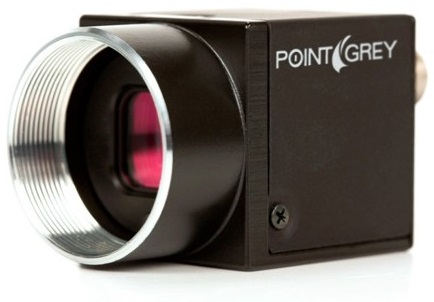
\includegraphics[height=0.25\columnwidth]{figs/Flea2.jpg}}\qquad
\subfloat{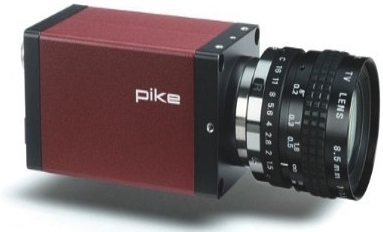
\includegraphics[height=0.25\columnwidth]{figs/Pike2.jpg}}
\caption{Câmeras utilizadas no TerraMax: Flea 2 (WGA) e Pike 2 (HD).}%
\label{fig:cameras}%
\end{figure}

As duas câmeras HD são utilizadas no sistema de visão lateral, sendo cada uma posicionada em um lado do veículo. Três câmeras são usadas no sistema trinocular, quatro no sistema estéreo (duas frontais e duas traseiras) e duas no sistema traseiro, conforme disposto na \reffig{fig:vision}.

\begin{figure}[h]
\centering
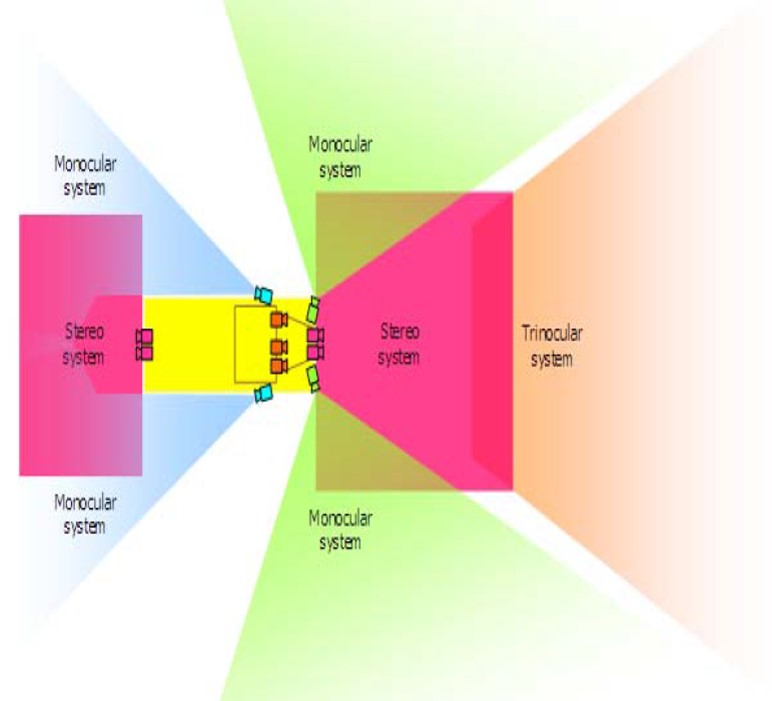
\includegraphics[width=0.75\columnwidth]{figs/vision.jpg}
\caption{Disposição das câmeras do sistema de visão.}%
\label{fig:vision}%
\end{figure}

\subsubsection{Visão Trinocular}

O sistema trinocular, que permite uma observação na faixa de 7 a 40m, é na verdade uma estratégia estéreo que pode ser chaveada em 3 diferentes \emph{baselines} (distância entre as duas câmeras). Com o veículo em velocidade baixa, é interessante utilizar o menor \emph{baseline}, mais preciso, enquanto com o veículo em alta velocidade, chaveia-se para o maior \emph{baseline}, que permite detecção de obstáculos a uma distância maior.

O objetivo desse subsistema de visão é a detecção de obstáculos à frente do veículo e a detecção das marcas da pista para controle de direção a médio e longo alcance. A escolha pelo sistema estéreo se fez porque ele permite uma reconstrução 3D do ambiente com razoável precisão sem conhecimento a priori do ambiente à frente do veículo.

O algoritmo utilizado na detecção de obstáculos inicia-se na retificação das imagens estéreo de forma a tornar as linhas epipolares horizontais, corrigindo possíveis desalinhamentos e erros de calibração das câmeras. Um mapa de disparidade ``V" extrai a inclinação da pista e do veículo para possíveis compensações durante oscilações. Então, um mapa de disparidade (diferença entre as duas imagens estéreo) é criado para realizar a detecção de obstáculos após uma filtragem da imagem correspondente ao veículo e imediatamente à sua frente. O restante do mapa de disparidade é então integrado com os scans dos LIDARs frontais para a detecção de objetos. O processo é ilustrado na \reffig{fig:trinocular_obstacle}.

\begin{figure}[h]
\centering
\subfloat[]{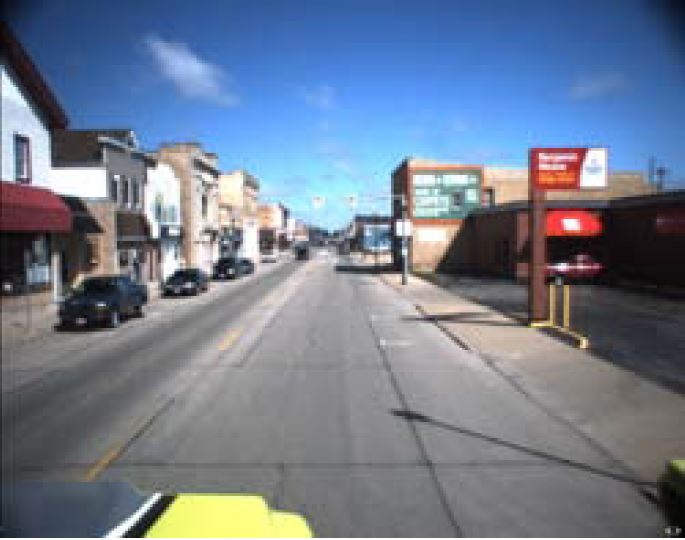
\includegraphics[height=0.275\columnwidth]{figs/trinocular_1.jpg}}\quad
\subfloat[]{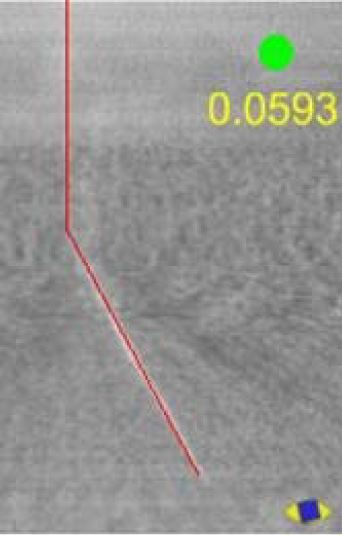
\includegraphics[height=0.275\columnwidth]{figs/trinocular_2.jpg}}\quad
\subfloat[]{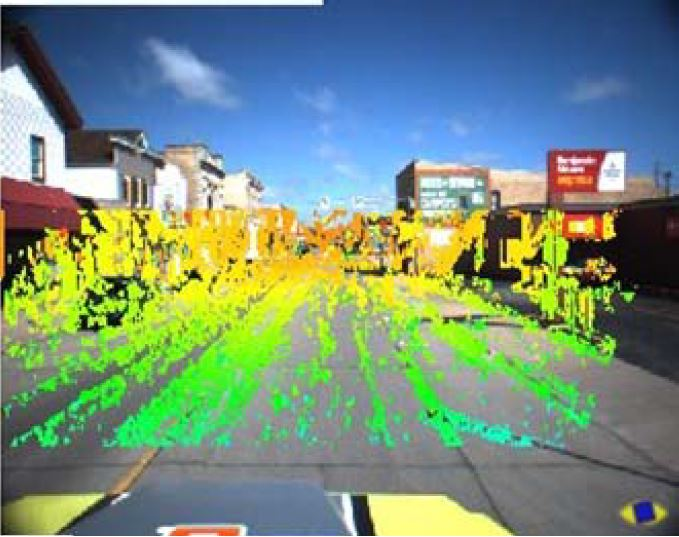
\includegraphics[height=0.275\columnwidth]{figs/trinocular_3.jpg}}
\caption{(a) Imagem original, (b) mapa de disparidade V com inclinação do veículo associada e (c) mapa de disparidade (pontos em verde próximos e em laranja mais afastados).}%
\label{fig:trinocular_obstacle}%
\end{figure}

As imagens estéreo são utilizadas também para detecção das faixas e limites das pistas. Inicialmente, a imagem é processada para remoção dos objetos detectados para diminuição de falsos positivos. Então, a imagem é duplicada e filtrada para predominância de branco em uma e amarelo na outra de modo a realizar a detecção das faixas brancas e amarelas. O efeito de perspectiva é então compensado através de uma transformação da imagem pelo mapeamento de perspectiva inversa, que leva em conta a inclinação da pista anteriormente estimada. Finalmente, é realizada uma busca de variações de luminância horizontal que permite detectar as faixas na imagem. O algoritmo possibilita detectar tanto faixas de diferente cor (amarelo e branco), como de diferente tipo (cheia ou listrada, simples ou dupla). Resultados desse processamento são mostrados na \reffig{fig:trinocular_lane}.

\begin{figure}[h]
\centering
\subfloat{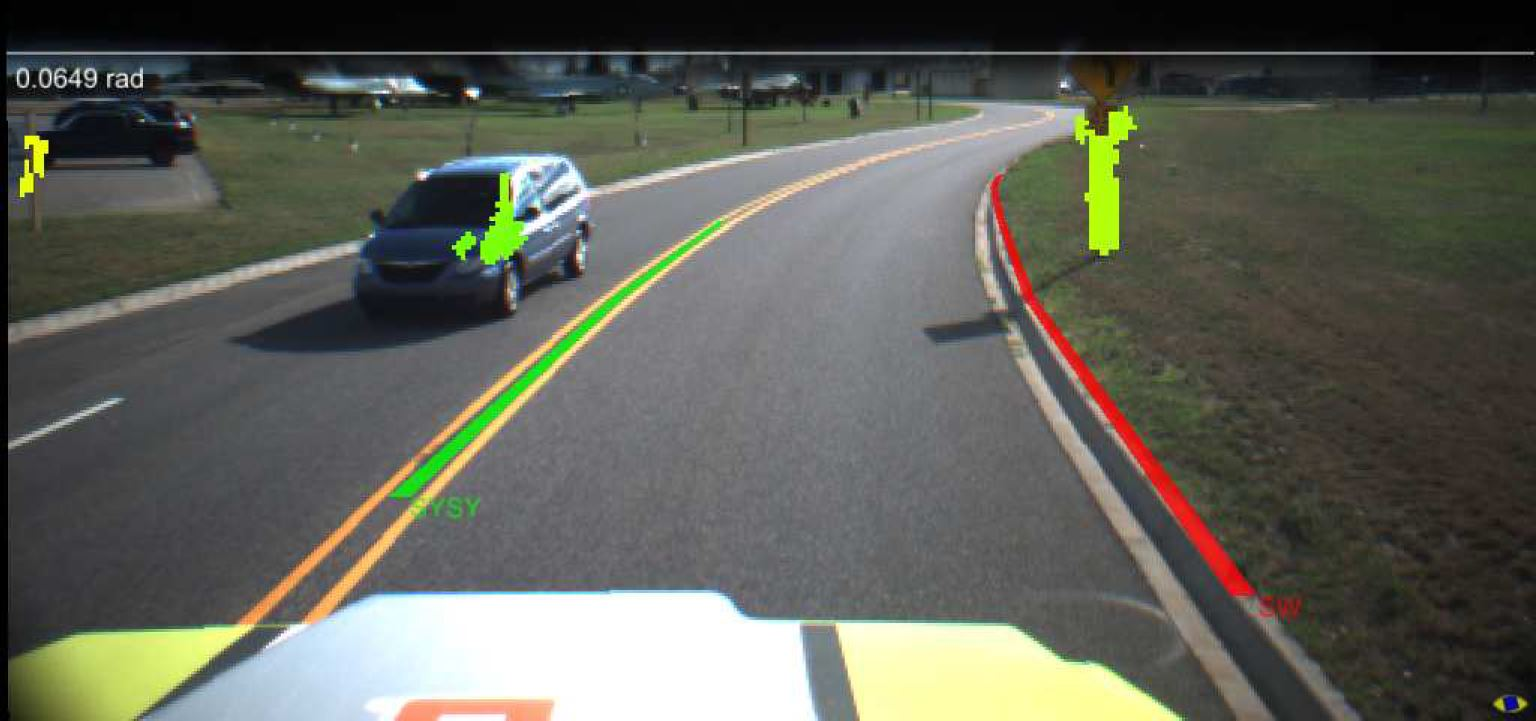
\includegraphics[height=0.225\columnwidth]{figs/trinocular_lane_2.jpg}}\quad
\subfloat{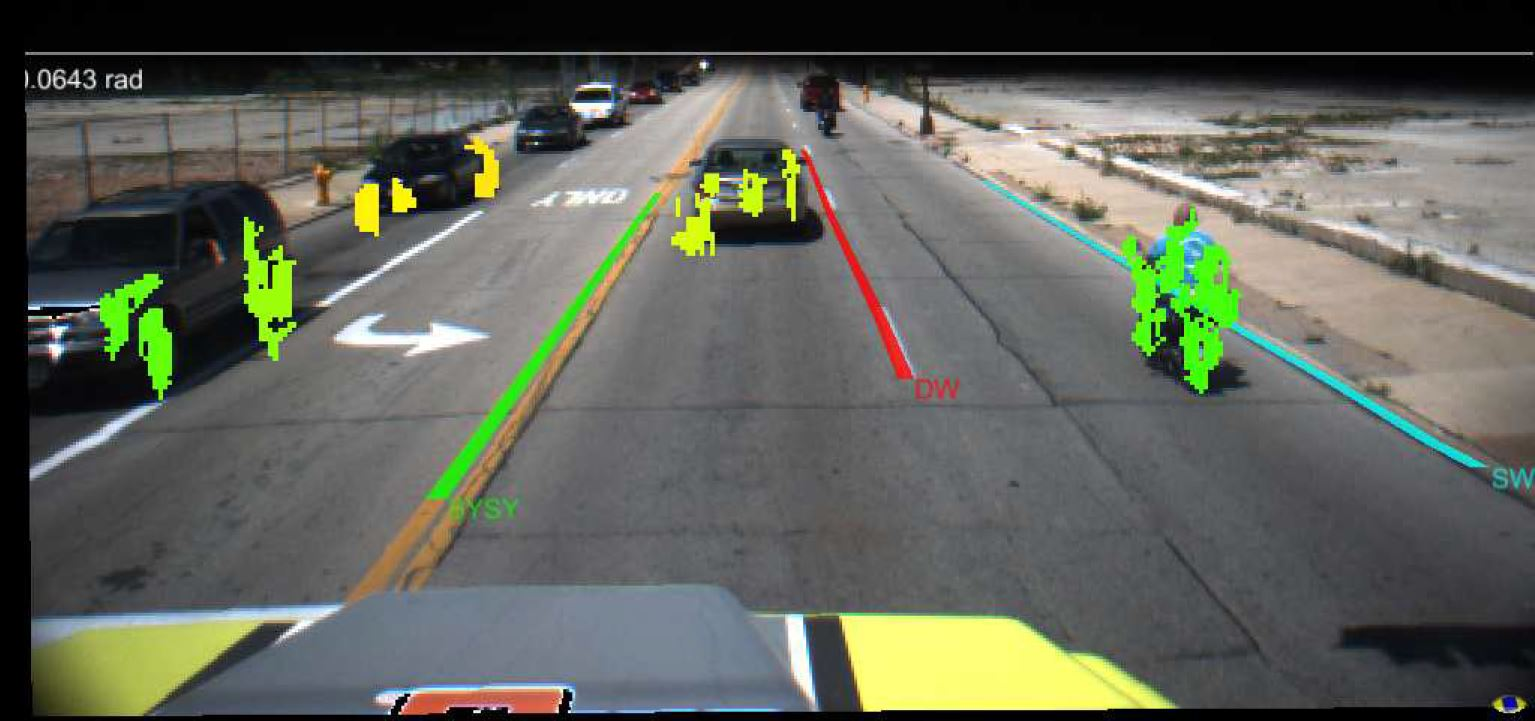
\includegraphics[height=0.225\columnwidth]{figs/trinocular_lane_3.jpg}}
\caption{Exemplos de detecção de faixas através do sistema trinocular.}%
\label{fig:trinocular_lane}%
\end{figure}

%Necessita de calibracao

\subsubsection{Visão Estéreo}

O subsistema estéreo do TerraMax possui duas câmeras frontais e duas traseiras apontadas em diagonal para o chão e possuem lentes \emph{fisheye} para ampliação do campo de visão ($\sim160\degree$) a uma área total de 10x10 metros. O objetivo é detectar obstáculos e faixas na pista próximos ao veículo com alta precisão e confiança. A ideia é aprimorar o sistema trinocular com a integração das informações dos dois subsistemas, já que faixas horizontais de parada em cruzamentos e faixas em curvas muito acentuadas não seriam detectadas pelo sistema trinocular, por exemplo.

A detecção de obstáculos é feita em dois passos. Primeiramente, as duas imagens estéreo são pré-processadas para remoção da distorção causada pela lente panorâmica e do efeito de perspectiva. Então, uma imagem diferencial é gerada e rotulada. Uma estratégia baseada em histogramas polares é utilizada para isolar os rótulos correspondentes aos obstáculos. Os dados dos LIDARs são também utilizados para melhorar a eficácia da detecção de objetos. Já a detecção de faixas utiliza a imagem de apenas uma câmera com um algoritmo semelhante ao utilizado no sistema trinocular. A \reffig{fig:stereo} mostra alguns resultados de detecção de obstáculos próximos e faixas.

\begin{figure}[h]
\centering
\subfloat{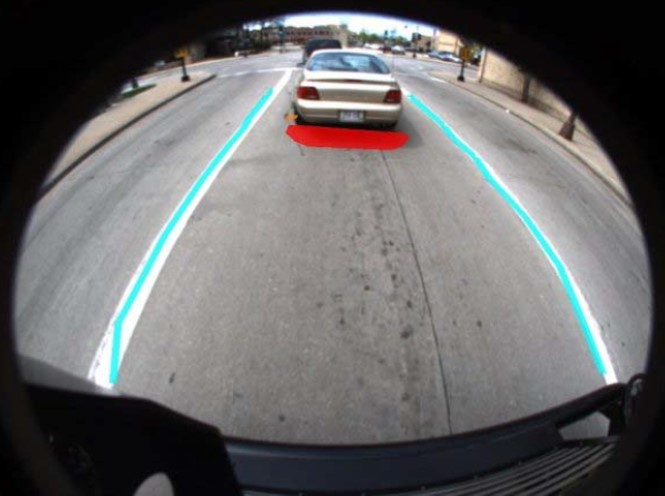
\includegraphics[height=0.235\columnwidth]{figs/stereo_1.jpg}}\quad
\subfloat{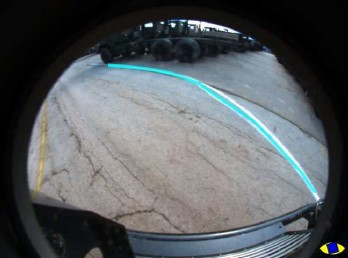
\includegraphics[height=0.235\columnwidth]{figs/stereo_2.jpg}}\quad
\subfloat{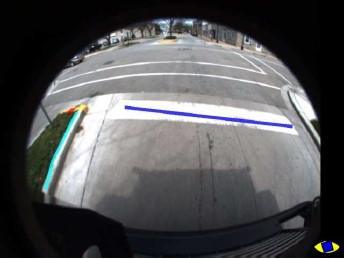
\includegraphics[height=0.235\columnwidth]{figs/stereo_3.jpg}}
\caption{Resultados de detecção de obstáculos e faixa do sistema estéreo.}%
\label{fig:stereo}%
\end{figure}

%The cameras setup selected for this system has the drawback of making it difficult to locate the exact boundaries of the detected items; to address this shortcoming, laser data is clustered and matched against the detected elements in the field of view, and when a correspondence is found the precise shape is sent to the World Perception Server. If no laser data is available, or the matching phase produces poor results, the system provides only the position of the obstacles, with no additional shape information.

\subsubsection{Visão Lateral}

O sistema de visão lateral é responsável por detectar a posição e velocidade dos veículos transitando por cruzamentos com um alcance de até 130 metros. Para reduzir o esforço computacional do processamento de imagens HD, o sistema só é ativado em situações de cruzamento. Além disso, a alta resolução é utilizada somente em determinada área de interesse, enquanto o restante é processado em uma resolução mais baixa.

A imagem é processada por um algoritmo robusto e \emph{ad-hoc} baseado em subtração de fundo em determinada região de interesse. A \reffig{fig:lateral} apresenta alguns resultados desse sistema de detecção.

\begin{figure}[h]
\centering
\subfloat{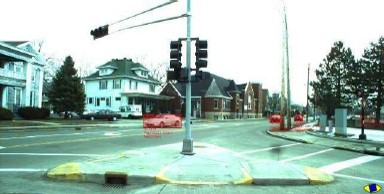
\includegraphics[height=0.24\columnwidth]{figs/lateral_1.jpg}}\quad
\subfloat{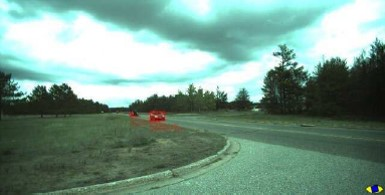
\includegraphics[height=0.24\columnwidth]{figs/lateral_2.jpg}}
\caption{Resultados de detecção de veículos pelo sistema de visão lateral.}%
\label{fig:lateral}%
\end{figure}

\subsubsection{Visão Traseira}

Através de duas câmeras instaladas na parte traseira e apontadas para trás do veículo, é possível detectar veículos que estejam fazendo ultrapassagem.

O algoritmo para detecção dos veículos é baseado em \emph{color clustering} e \emph{optical flow}. Primeiramente, porções da imagem ou objetos de cor uniforme são categorizados dependendo da cor dos pixels na imagem. Após isso, essas regiões são analisadas e rastreadas através de fluxo ótico (deslocamento de pixels ou regiões entre quadros consecutivos), estimando assim o contorno e o movimento desses objetos. As estimações também são refinadas com os dados dos LIDARs através de algoritmos de fusão sensorial. A \reffig{fig:rear} apresenta alguns resultados desse subsistema.

\begin{figure}[h]
\centering
\subfloat{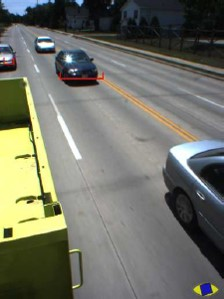
\includegraphics[height=0.3\columnwidth]{figs/rear_1.jpg}}\enskip
\subfloat{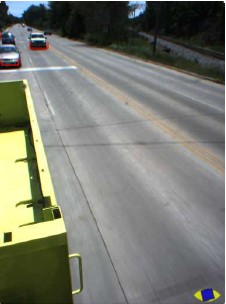
\includegraphics[height=0.3\columnwidth]{figs/rear_2.jpg}}\enskip
\subfloat{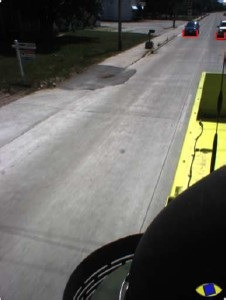
\includegraphics[height=0.3\columnwidth]{figs/rear_3.jpg}}\enskip
\subfloat{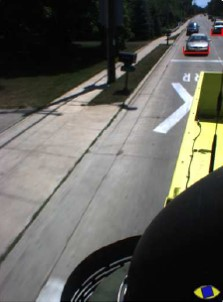
\includegraphics[height=0.3\columnwidth]{figs/rear_4.jpg}}
\caption{Resultados de detecção de veículos pelo sistema de visão traseira.}%
\label{fig:rear}%
\end{figure} 